\documentclass[letterpaper, 12pt]{article}
\usepackage{geometry}
\geometry{
    letterpaper,
    left=20mm,
    top=20mm,
    bottom=20mm
}
\usepackage{tocloft}
\usepackage{graphicx}
\usepackage{authblk}
\usepackage{amssymb}
\usepackage{lipsum}
\usepackage{float}
\usepackage{times}
\usepackage{amsmath}
\usepackage[format=plain,
            labelfont={bf,it},
            textfont=it]{caption}
\captionsetup{justification=raggedright,singlelinecheck=false}
\usepackage{ragged2e}
\usepackage{longtable}
\usepackage{comment}
\usepackage{setspace}
\usepackage{fancyhdr}
\usepackage{titlesec}
\usepackage[hyperindex,breaklinks]{hyperref}
\hypersetup{
    colorlinks=true,
    linkcolor=blue,
    filecolor=magenta,      
    urlcolor=blue
}
\usepackage[T1]{fontenc}
\usepackage{helvet}
\renewcommand{\familydefault}{\sfdefault}
\pagenumbering{gobble}
\usepackage[skip=10pt plus1pt, indent=40pt]{parskip}
\usepackage{orcidlink}
\usepackage{standalone}

\titlespacing*{\section}
{0pt}{1.5ex plus 1ex minus .2ex}{1.3ex plus .2ex}

\renewcommand\Authfont{\fontsize{12}{14.4}\selectfont}
\renewcommand\Affilfont{\fontsize{9}{10.8}\itshape}

\newcommand{\cosigpart}[1]{
  \addcontentsline{toc}{part}{#1}
}
\newcommand{\cosigsection}[1]{
  \section*{#1}
  \phantomsection % avoid warnings from hyperref about the anchor of a bookmark and its parent's
  \addcontentsline{toc}{section}{#1}
}
\begin{document}
\flushleft
\includegraphics[width=0.5\textwidth]{img/home/241017_final_logo_mockup.png}

\cosigsection{Image compression artifacts}
\textit{Last updated: 4 June 2025}

Image files are often \href{https://en.wikipedia.org/wiki/Data_compression}{compressed} to take up less disk space. Lossy compression algorithms like \href{https://en.wikipedia.org/wiki/JPEG}{JPEG} often leave visual artifacts in the compressed image, including:

\begin{itemize}
    \setlength\itemsep{-0.5em}
    \item \textbf{``Blocks'' appearing in the image.} These blocks appear as sharp vertical and horizontal transitions and are introduced by JPEG's application of the \href{https://en.wikipedia.org/wiki/Discrete_cosine_transform}{discrete cosine transform} algorithm. These blocks can appear superficially similar to ``splicing'' artifacts indicative of image manipulation (see COSIG's \href{https://osf.io/547re}{entry on image duplication}).
    \item \textbf{\href{https://en.wikipedia.org/wiki/Ringing_artifacts}{``Ringing''} artifacts around sharp transitions in the image.} These artifacts are especially apparent surrounding graphs and text.
    \item \textbf{Distortion of colors and introduction of new colors into an image.}
\end{itemize}

\begin{figure}[h!tbp]
    \centering
    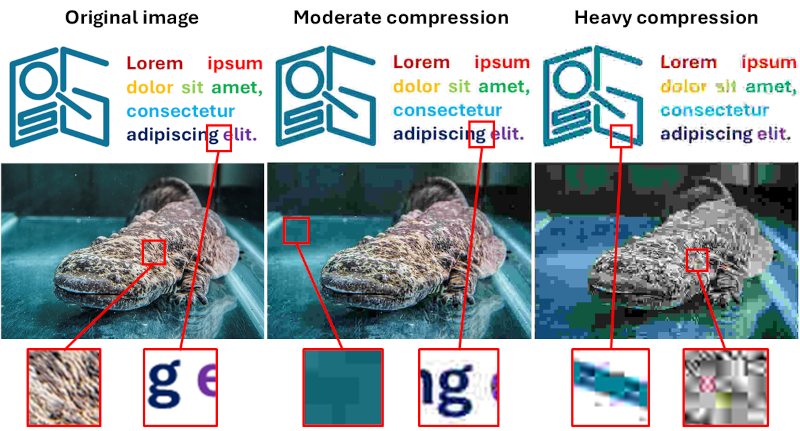
\includegraphics[width=\textwidth]{img/compression_artifacts/image_compression_fig_small.png}
    \caption*{The same figure (original on left) subjected to moderate JPEG compression (middle, Q=10) and heavy JPEG compression (right, Q=0). Various compression artifacts are highlighted with red boxes below the figure.}
\end{figure}

The presence of image compression artifacts is, by itself, not an indication of image manipulation. On the other hand, sometimes duplications can be obscured by compression artifacts. If the image quality is low in a suspected duplication or one of the two images is more affected by lossy compression, the two images may no longer be pixel-identical. Images that are not pixel-identical can still be considered duplications if they appear too similar to genuinely depict different subjects.

If you are unsure if an image feature is due to image compression, try to see if there are other compression artifacts present in the image. To investigate potential image duplications, it is always preferable to assess the original, uncompressed image files.

\subsection*{Additional resources}

\begin{itemize}
    \setlength\itemsep{-0.5em}
    \item \href{https://osf.io/547re}{COSIG: Image duplication}
    \item \href{https://doi.org/10.1007/s11263-022-01617-5}{``Learning JPEG Compression Artifacts for Image Manipulation Detection and Localization'' (2022)}
\end{itemize}

\end{document}